\documentclass[class=../../report, crop=false]{standalone}
\usepackage{graphicx}
\usepackage{mathtools}
\usepackage{float}
\usepackage{pgfplots}

\newcommand{\msii}{\frac{\text{m}}{\text{s}^2}}
\newcommand{\kgmiii}{\frac{\text{kg}}{\text{m}^3}}

\begin{document}

\section{Prototype Tests} \label{app:prototypetests}
\subsection{Feasibility Calculation for Fan Propulsion} \label{app/sub:fan}

The force required to move is greater than the frictional force of the train:
\begin{align}
	F > \mu mg
\end{align}
We assume our train will have $m \approx 0.5\text{kg}$\footnotemark and  $\mu_s \approx 0.6$
\footnotetext{A cargo cart is 450g unloaded, this assumes we will carry roughly 50g of cargo}
\begin{align}
	F &= (0.6)(0.5\text{kg})\left(10\msii\right) \\
	  &= 3\text{N}
\end{align}
The force from the fan can be found using the following formula assuming the motor has a maximum power output of 19W (Mabuchi Motors, 2018).
\begin{align}
	P &= \sqrt{\frac{F^3}{2\rho A}}
\end{align}
Solving for area:
\begin{align}
	A &= \frac{F^3}{2\rho P^2} \\
	  &= \frac{\left(3\text{N}\right)^3}{2\left(1.225\kgmiii\right)\left(19\text{W}\right)^2} \\
	  &= 0.03\text{m}^2
\end{align}
Assuming the fan sqeeps a circular path:
\begin{align}
	A &= \pi r^2 \\
	r &= \sqrt{\frac{A}{\pi}} \\
	r &= 0.10\text{m}
\end{align}
Our train must have a height smaller than 6'' (15.24cm) above the rails.
The diameter of the fan is too large to fit within this restriciton.

\clearpage

\subsection{Wheel Testing}
\begin{table}[H]
	\centering
	\begin{tabular}{l | l}
		Prototype design & Number of derails \\ \hline
		Conical wheels, low CoG & 2 \\
		Cylindrical wheels, low CoG & 5 \\
		Conical wheels, high CoG & 9 \\
	\end{tabular}

	\caption{Wheel Design Test Results}
	\label{app/table:wheeltest}
\end{table}

We decided to test the wheel shapes due to the emphasis on stability in our strategy.
We tested the wheel designs using the following procedure:
\begin{enumerate}
	\item Create chassis with various centeres of gravity
	\item Combine chassis designs with cylindrical or conical wheels
	\item Release chassis from top of slope towards a corner
	\item Record number of derailments across 9 trials
\end{enumerate}

\clearpage

\subsection{Calculation of Dual Drive Torque} \label{app/sub:dualdrivetorque}

We needed to compare the use of multiple motors to the use of a single motor.
We used a simple calculation since this was much faster than creating a physical prototype.
We compared a single motor and two motors in parallel (Figure \ref{app/fig:motorcomp}).

\begin{figure}[H]
	\centering
	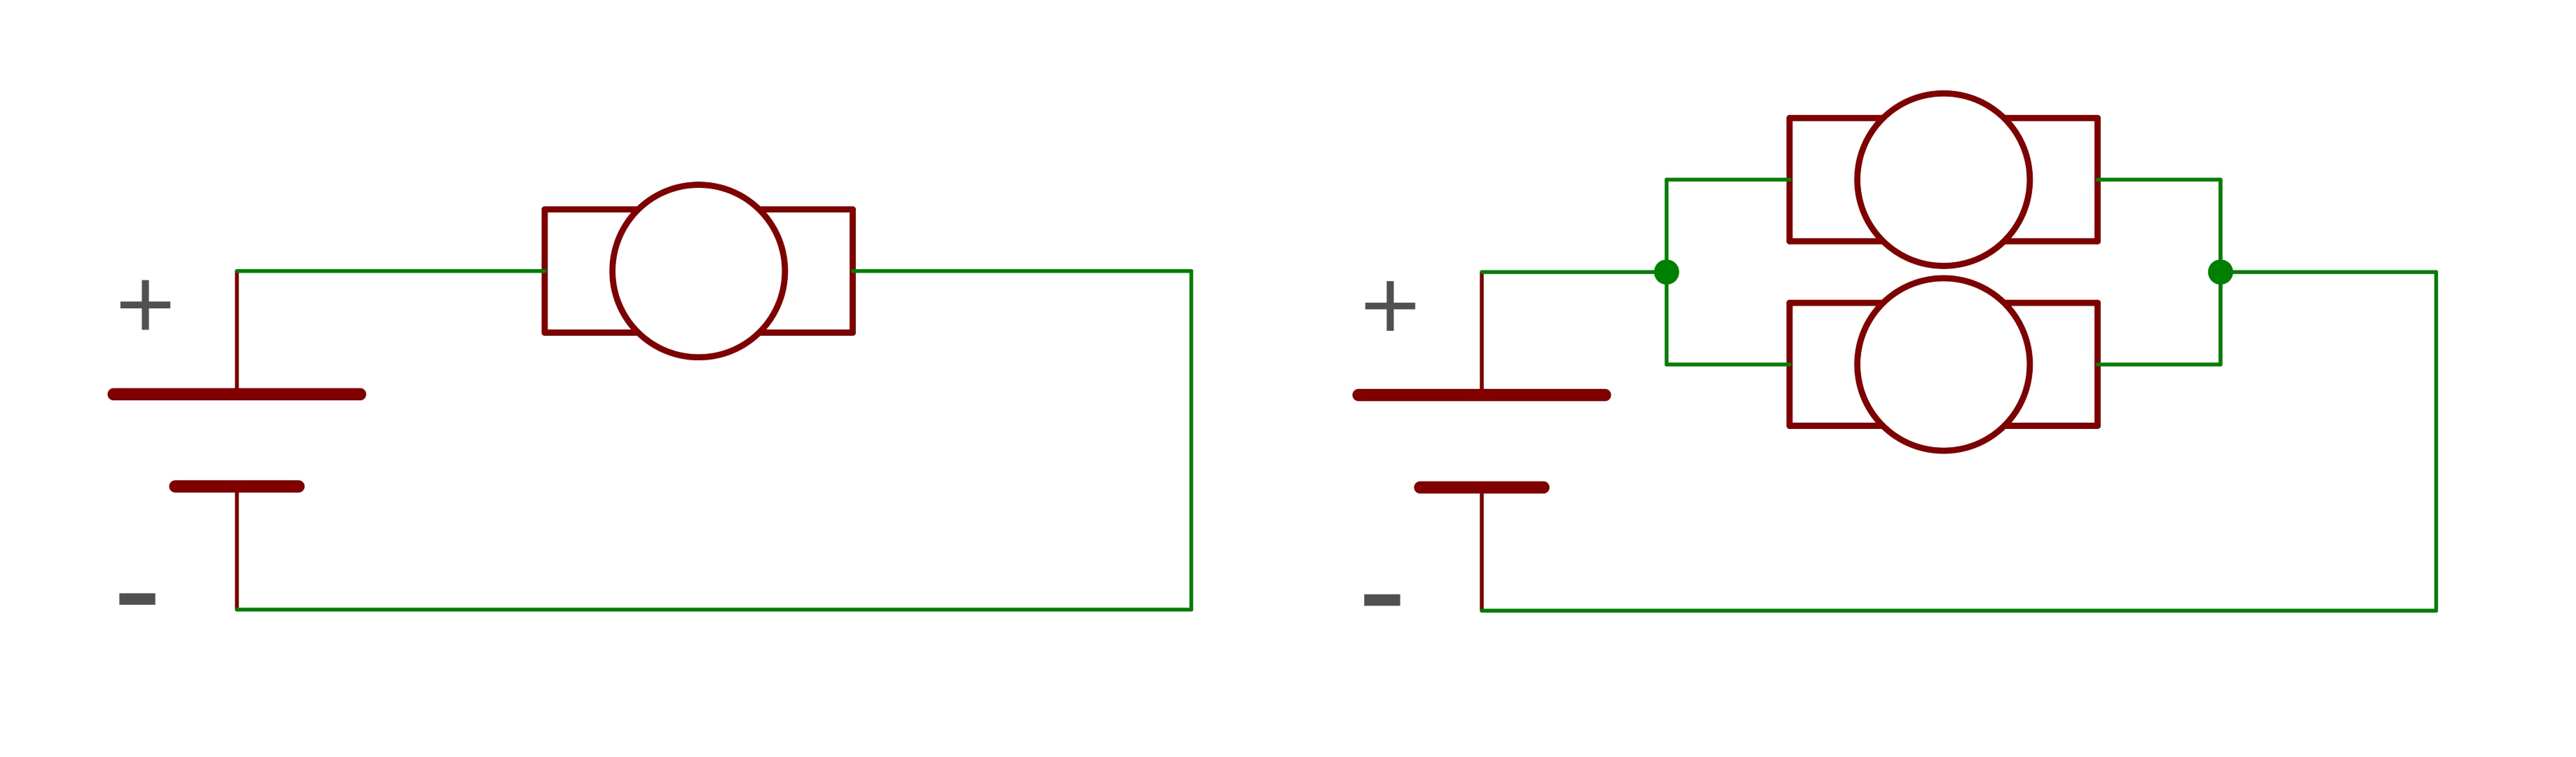
\includegraphics[width=0.8\textwidth]{../../res/img/motorcomp}
	\caption{Possible Motor Configurations}
	\label{app/fig:motorcomp}
\end{figure}

If we can assume the two DC motors provide the same resistance in phase, then the total resistance will be half of the resistance when flowing through only one motor.
This means the total current running through the source is double that of the current when only one motor is attached.
The current in branch is the same (by Kirchhoff’s Current Law) and each motor outputs the same torque as the single motor.
Since we now have two motors, the total torque is twice that of a single motor.

By this logic, so long as other factors do not have a significant negative impact on our design, there is no disadvantage to using multiple motors provided our battery life is sufficient.

\clearpage

\subsection{Calculation of Prototype Torque}
\begin{table}[H]
	\centering
	\begin{tabular}{l | l}
		Mass & Max incline climbed\\ \hline
		0.589kg & 22$^{\circ}$ \\
	\end{tabular}

	\label{app/table:torquetest}

	\caption{Torque Test Data}
\end{table}

This test was conducted to determine if the train could exert sufficient torque to push itself up the incline or if it could pull cargo as well.
The train was placed on the track and the motor turned on.
We began increasing the incline of the track until the motor stalled.
We recorded this maximum incline for the prototype, and weighed the prototype.
Using this data, we calculated the max torque output of the motor.
\begin{align}
	F_{x'} &= ma_{x'} \\
	a_{x'} &= 0 \left(\text{static}\right) \\
	F_{x'} &= mg \sin{\theta} - F_{\text{motor}} \\
	\frac{T_{\text{motor}}}{r_{\text{wheel}}} &= mg \sin{\theta} \\
	T_{\text{motor}} &= mg \sin{\theta} * r_{\text{wheel}} \\
	T_{\text{motor}} &= \left(0.589\text{kg}\right)\left(9.81\msii\right) \sin{22^{\circ}} * 0.015\text{m} \\
	T_{\text{motor}} &= 32.5\text{mN}*\text{m}
\end{align}

This output was much lower than we expected.
We needed to increase the gear ratio we were using or we needed to add motors to increase the amount of torque supplied.

\clearpage

\subsection{Frictional Data Test}

We determined the coefficient of static friction of our wheels to determine the maximum amount of force that could be used.
We locked the wheels of our train prototype and placed it on a slope with a variable incline.
We varied the angle of the slope until the train began to slip, then we used the following equations to calculate a value for the coefficient of friction.

\begin{align}
	F_{x'} &= ma_{x'} \\
	a_{x'} &= 0 \left(\text{static}\right) \\
	F_{x'} &= mg \sin{\theta} - \mu mg \cos{\theta} = 0 \\
	g \sin{\theta} &= \mu g \cos{\theta} \\
	\mu &= \tan{\theta}
\end{align}

\begin{table}[H]
	\centering
	\begin{tabular}{l | l l l}
		 & PLA & Rubber coating & Rubber band \\ \hline
		$\theta$(degrees) & 9.64 & 35 & 52.4 \\
		$\mu$ & 0.17 & 0.7 & 1.3 \\
	\end{tabular}

	\caption{Static Coefficient of Friction Data}
	\label{app/table:staticcoeff}
\end{table}

The drastic increase in friction demonstrated that we needed to use a cover on our wheels, and it showed that the rubber band would be best for this purpose.

\clearpage

\subsection{Light Sensor Test} \label{app/sub:photores}
In order to test the feasibility of using a light sensor to count track ties we attached it to the bottom of our train with two LEDs to illuminate the tracks.

\begin{figure}[H]
	\centering
	\begin{tikzpicture}
		\begin{axis}[
				title={\textbf{Photo Resistor Data}},
				width=0.8\textwidth,
				height=0.45\textwidth,
				ymajorgrids,
				xmin=1,
				xmax=313,
				xticklabels={,,},
				xlabel={Time},
				ylabel={Luminosity}
			]
			\addplot table[x=t,y=val, col sep=comma,mark=none]{lightsensor.csv};
		\end{axis}
	\end{tikzpicture}
	% Specify title without footnotemark for list of figures
	\caption[Photoresistor Track Detection Data]{Photoresistor Track Detection Data\protect\footnotemark}
	\label{app/fig:photores}
\end{figure}
\footnotetext{The axes lack dimensions because they are raw values taken from an Arduino}

This physical test allowed us to determine if the photoresistor would be able to differentiate between the track ties.
The data above shows the peaks and troughs as the prototype passed over the rails.
They become closer together as the prototype accelerated.
This test demonstrated that our braking system was feasible since it was possible for an Arduino to count the number of track ties is passes from this data.

\clearpage

\subsection{Track Simulation} \label{app/sub:tracksimulation}

We wanted to test the parameters of our prototype on the tracks.
Without access to the course, we decided to create a simulation that completed the following tasks (Figure \ref{app/fig:simflow}) to model the prototype completing the track.

\begin{figure}[H]
	\centering
	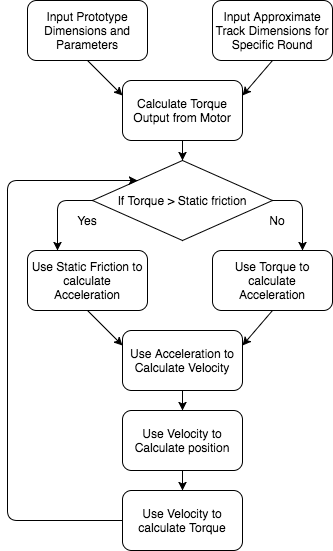
\includegraphics[width=0.6\textwidth]{../../res/img/simflow}
	\caption{Simulation Flow Chart}
	\label{app/fig:simflow}
\end{figure}

The algorithm above was repeated until the train completed the length of track for the round, and the results were plotted.
Our simulation showed that the prototype reached a speed much higher than the calculated tipping velocity of 1.2m/s (Desmos Graphing Calculator, 2018).
This demonstrated that we needed to use a braking system to reduce our speed going into corners.

\end{document}
